\documentclass[12pt]{beamer}
\usetheme{Boadilla}
\usepackage{booktabs}
\usepackage{multirow}
\usepackage{enumitem}
\usepackage{tikz}
\usepackage[normalem]{ulem} 
\newcommand{\E}{\mathbb{E}}
\usefonttheme{professionalfonts}
\usepackage{pgfplots}
\pgfplotsset{compat=1.18}
\renewcommand{\arraystretch}{1.25}
\usetikzlibrary{trees}
\title[ECON2843]{Lecture 27}
\subtitle{Part 6 Introduction to Bayesian Statistics}
\date{}
\usepackage{amsmath,amssymb,mathtools,wasysym}
\begin{document}
	\begin{frame}
		\titlepage
		
	\end{frame}
		\begin{frame}
		\vspace{1cm}
		\centering
		{\color{blue}\large Bayesian Inference}
	\end{frame}
\begin{frame}
	\frametitle{Bayesian Inference}
	
	\begin{itemize}[label={\color{blue}$\blacktriangleright$}]
		\item Now for something completely different.
		
		\item Everything we have done up to now is frequentist statistics.
		Bayesian statistics is very different.
		
		\item Bayesians don't do confidence intervals and hypothesis tests.
		Bayesians don't use sampling distributions of estimators. Modern
		Bayesians aren't even interested in point estimators.
		
		\item So what do they do? Bayesians treat parameters as random
		variables.
			\end{itemize}
	\end{frame}
\begin{frame}
	\frametitle{Bayesian Inference}
	\begin{itemize}[label={\color{blue}$\blacktriangleright$}]
		\item To a Bayesian probability is the only way to describe uncertainty.
		\item Things not known for certain --- like values of parameters ---
		must be described by a probability distribution.
	\end{itemize}
	
\end{frame}
\begin{frame}
	\frametitle{Bayesian Inference}
	
	\begin{itemize}[label={\color{blue}$\blacktriangleright$}]
		\item Suppose you are uncertain about something. Then your uncertainty is described by a probability distribution called your \textit{prior distribution}.
		
		\item Suppose you obtain some data relevant to that thing. The data changes your uncertainty, which is then described by a new probability distribution called your \textit{posterior distribution}.
		
		\item The posterior distribution reflects the information both in the prior distribution and the data.
		
		\item Most of Bayesian inference is about how to go from prior to posterior.
	\end{itemize}
	
\end{frame}
\begin{frame}
	\frametitle{Bayesian Inference}
	
	\begin{itemize}[label={\color{blue}$\blacktriangleright$}]
		\item The way Bayesians go from prior to posterior is to use the laws of conditional probability, sometimes called in this context \textit{Bayes rule} or \textit{Bayes theorem}.
		
		\item Suppose we have a PDF $g$ for the prior distribution of the parameter $\theta$, and suppose we obtain data $x$ whose conditional PDF given $\theta$ is $f$. Then the joint distribution of data and parameters is conditional times marginal
		\[ f(x|\theta)g(\theta) \]
		It is a generalized form of $P(B|A)P(A)$ we have seen.

	\end{itemize}
	
\end{frame}
\begin{frame}
	\frametitle{Bayesian Inference}
	
	\begin{itemize}[label={\color{blue}$\blacktriangleright$}]
		\item The correct posterior distribution, according to the Bayesian paradigm, is the conditional distribution of $\theta$ given $x$, which is joint divided by marginal
		
		\[ h(\theta|x) = \frac{f(x|\theta)g(\theta)}{\int f(x|\theta)g(\theta)\,d\theta} \]
		
		\item Often we do not need to do the integral. If we recognize that
		\[ \theta \mapsto f(x|\theta)g(\theta) \]
		is, except for constants, the PDF of a brand name distribution, then that distribution must be the posterior.
	\end{itemize}
	
\end{frame}
\begin{frame}
	\frametitle{Bayes' Theorem}
	
	\begin{itemize}[label={\color{blue}$\blacktriangleright$}]
		\item Bayes' Theorem is about conditional probability.
		
		\item It has statistical applications.
	\end{itemize}
	
\end{frame}
\begin{frame}
	\frametitle{Conditional Probability}
	
\centering
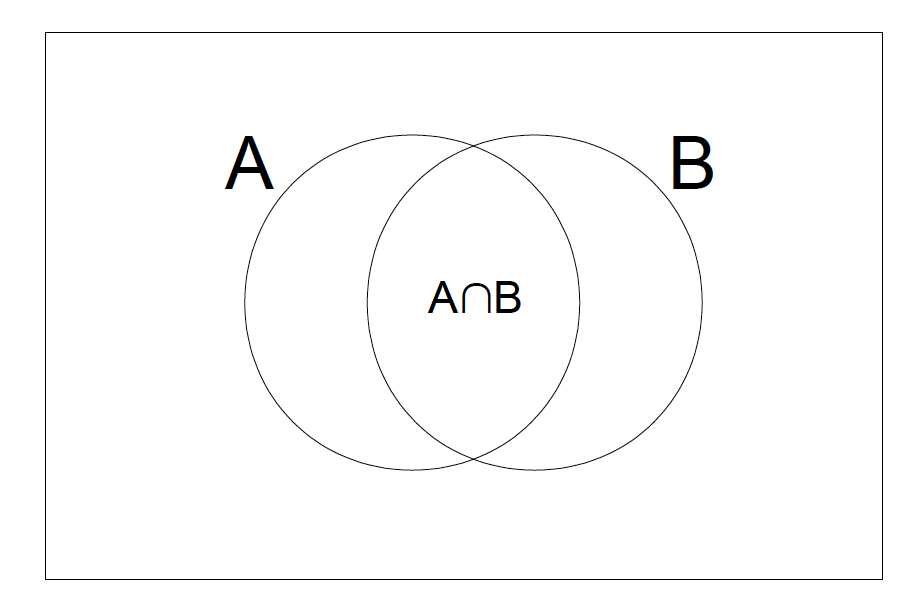
\includegraphics[width=10cm]{bayes.png}
$$P(A|B)=\frac{P(A\cap B)}{P(B)}$$

	
\end{frame}
\begin{frame}
	\frametitle{Multiplication Rule}
	
	\[
	\text{From }P(A|B) = \frac{P(A\cap B)}{P(B)}\text{, get }P(A\cap B) = P(A|B)P(B).
	\]
	
	\[
	\text{From }P(B|A) = \frac{P(B\cap A)}{P(A)}\text{, get }P(A\cap B) = P(B|A)P(A)
	\]
	
\end{frame}
\begin{frame}
	\frametitle{Bayes' Theorem}
	\framesubtitle{The most elementary version}
	\centering
	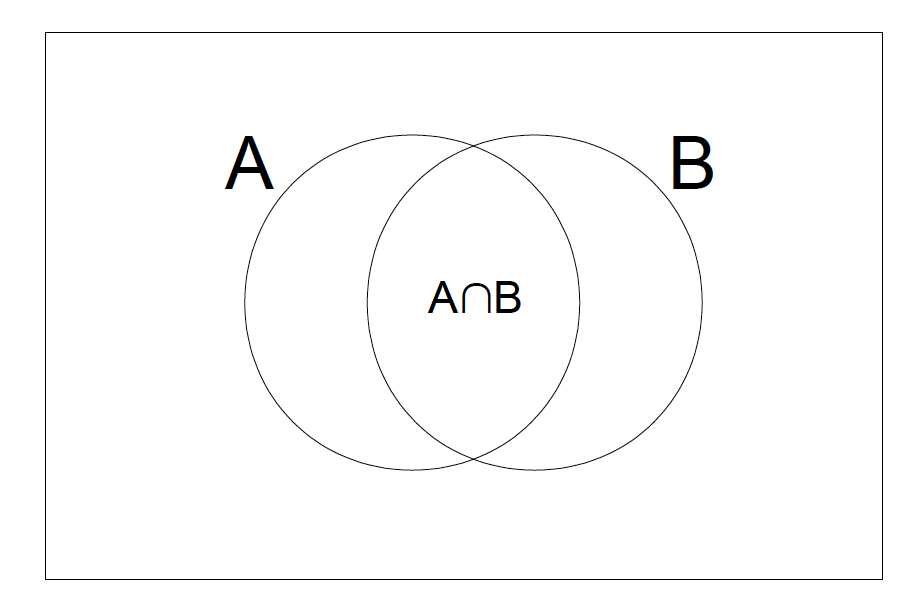
\includegraphics[width=5cm]{bayes.png}
	\[
	\begin{aligned}
		P(A|B) &= \frac{P(A\cap B)}{P(B)} \\
		&= \frac{P(A\cap B)}{P(A\cap B) + P(A^c\cap B)} \\
		&= \frac{P(B|A)P(A)}{P(B|A)P(A) + P(B|A^c)P(A^c)}
	\end{aligned}
	\]
	
\end{frame}
\begin{frame}
	\frametitle{Define ``events'' in Terms of Random Variables}
	\framesubtitle{Instead of $A$, $B$, etc.}
	
	\[
	P(Y = y|X = x) = \frac{P(X = x, Y = y)}{P(X = x)}
	\]
	
\end{frame}
\begin{frame}
	\frametitle{Continuous Random Variables}
	
	We have conditional densities:
	
	\[
	f_{y|x}(y|x) = \frac{f_{xy}(x,y)}{f_x(x)}
	\]
	
\end{frame}
\begin{frame}
	\frametitle{Different Versions of Bayes' Theorem}
	
	For discrete random variables,
	
	\[
	\begin{aligned}
		P(X = x|Y = y) &= \frac{P(X = x, Y = y)}{P(Y = y)} \\[1em]
		&= \frac{P(Y = y|X = x)P(X = x)}{\sum_t P(Y = y|X = t)P(X = t)}
	\end{aligned}
	\]
	
\end{frame}
\begin{frame}
	\frametitle{Continuous Random Variables}
	
	\[
	\begin{aligned}
		f_{x|y}(x|y) &= \frac{f_{xy}(x,y)}{f_y(y)} \\[1em]
		&= \frac{f_{y|x}(y|x)f_x(x)}{\int f_{y|x}(y|t)f_x(t)\,dt}
	\end{aligned}
	\]
	
\end{frame}
\begin{frame}
	\frametitle{Compare}
	
	\[
	\begin{aligned}
		P(A|B) &= \frac{P(B|A)P(A)}{P(B|A)P(A) + P(B|A^c)P(A^c)} \\[2em]
		P(X = x|Y = y) &= \frac{P(Y = y|X = x)P(X = x)}{\sum_t P(Y = y|X = t)P(X = t)} \\[2em]
		f_{x|y}(x|y) &= \frac{f_{y|x}(y|x)f_x(x)}{\int f_{y|x}(y|t)f_x(t)\,dt}
	\end{aligned}
	\]
	
\end{frame}
\begin{frame}
	\frametitle{Philosophy}
	\framesubtitle{Bayesian versus Frequentist}
	
	\begin{itemize}[label={\color{blue}$\blacktriangleright$}]
		\item What is probability?
		
		\item Probability is a formal axiomatic system.
		
		\item \textit{Of what} is probability a model?
	\end{itemize}
	
\end{frame}
\begin{frame}
	\frametitle{\textit{Of what} is Probability a Model?}
	\framesubtitle{Two answers}
	
	\begin{itemize}[label={\color{blue}$\blacktriangleright$}]
		\item Frequentist: Probability is long-run relative frequency.
		
		\item Bayesian: Probability is degree of subjective belief.
	\end{itemize}
	
\end{frame}
\begin{frame}
	\frametitle{Statistical Inference}
	\framesubtitle{How it works}
	
	\begin{itemize}[label={\color{blue}$\blacktriangleright$}]
		\item Adopt a probability model for data set $Y$.
		
		\item Distribution of $Y$ depends on a parameter $\theta$.
		
		\item Use observed value $Y = y$ to decide about $\theta$.
		
		\item Translate the decision into a statement about the process that generated the data.
		
		\item Bayesians and Frequentists agree so far, mostly.
		
		\item The description above is limited to what frequentists can do.
		
		\item Bayes methods can generate more specific recommendations.
	\end{itemize}
	
\end{frame}
\begin{frame}
	\frametitle{What is a Parameter?}
	
	\begin{itemize}[label={\color{blue}$\blacktriangleright$}]
		\item To the frequentist, it is an unknown constant.
		
		\item To the Bayesian since we don't know the value of the parameter, it's a random variable.
	\end{itemize}
	
\end{frame}
\begin{frame}
	\frametitle{Unknown Parameters are Random Variables}
	\framesubtitle{To the Bayesian}
	
	\begin{itemize}[label={\color{blue}$\blacktriangleright$}]
		\item That's because probability is subjective belief.
		
		\item We model our uncertainty with a probability distribution, $\pi(\theta)$.
		
		\item $\pi(\theta)$ is called the \textit{prior} distribution.
		
		\item Prior because it represents the statistician's belief about $\theta$ \textit{before} observing the data.
		
		\item The distribution of $\theta$ after seeing the data is called the \textit{posterior} distribution.
		
		\item The posterior is the conditional distribution of the parameter given the data.
	\end{itemize}
	
\end{frame}
\begin{frame}
	\frametitle{Bayesian Inference}
	
	\begin{itemize}[label={\color{blue}$\blacktriangleright$}]
		\item Model is $p(x|\theta)$ or $f(x|\theta)$.
		
		\item Prior distribution $\pi(\theta)$ is based on the best available information.
		
		\item But yours might be different from mine. It's subjective.
		
		\item Use Bayes' Theorem to obtain the posterior distribution $\pi(\theta|x)$.
		
		\item As the notation indicates, $\pi(\theta|x)$ might be the prior for the next experiment.
	\end{itemize}
	
\end{frame}
\begin{frame}
	\frametitle{Subjectivity}
	
	\begin{itemize}[label={\color{blue}$\blacktriangleright$}]
		\item Subjectivity is the most frequent objection to Bayesian methods.
		
		\item The prior distribution influences the conclusions.
		
		\item Two scientists may arrive at different conclusions from the same data, \textit{based on the same statistical analysis}.
		
		\item The influence of the prior goes to zero as the sample size increases
		
	\end{itemize}
	
\end{frame}
\begin{frame}
	\frametitle{Bayes' Theorem}
	\framesubtitle{Continuous case}
	
	\[
	\pi(\theta|x) = \frac{f(x|\theta)\pi(\theta)}{\int f(x|t)\pi(t)\,dt}
	\]
	
	
	\[
	\propto f(x|\theta)\pi(\theta)
	\]
	
\end{frame}
\begin{frame}
	\frametitle{Once You Have the Posterior Distribution, You Can \ldots}
	
	\begin{itemize}[label={\color{blue}$\blacktriangleright$}]
		\item Give a point estimate of $\theta$. Why not $E(\theta|X = x)$?
		
		\item Test hypotheses, like $H_0 : \theta \in H$.
		
		\item Reject $H_0$ if $P(\theta \in H|X = x) < P(\theta \notin H|X = x)$. \\ Why not?
		
		\item We should be able to do better than ``Why not?''
	\end{itemize}
	
\end{frame}
\begin{frame}
	\frametitle{Decision Theory}
	
	\begin{itemize}[label={\color{blue}$\blacktriangleright$}]
		\item Any time you make a decision, you can lose something.
		
		\item Risk is defined as expected loss.
		
		\item Goal: Make decisions so as to minimize risk.
		
		\item Or if you are an optimist, you can maximize expected utility.
	\end{itemize}
	
\end{frame}
\begin{frame}
	\frametitle{Decisions}
	
	\[
	d = d(x) \in \mathcal{D}
	\]
	
	\begin{itemize}[label={\color{blue}$\blacktriangleright$}]
		\item $d$ is a decision.
		
		\item It is based on the data.
		
		\item It is an element of a \textit{decision space}.
	\end{itemize}
	
\end{frame}
\begin{frame}
	\frametitle{Decision Space $\mathcal{D}$}
	
	\begin{itemize}[label={\color{blue}$\blacktriangleright$}]
		\item It is the set of possible decisions that might be made based on the data.
		
		\item For estimation, $\mathcal{D}$ is the parameter space.
		
		\item For accepting or rejecting a null hypothesis, $\mathcal{D}$ consists of 2 points.
		
		\item Other kinds of kinds of decision are possible, not covered by frequentist inference.
		
		\item What kind of chicken feed should the farmer buy?
	\end{itemize}
	
\end{frame}
\begin{frame}
	\frametitle{Loss Function}
	
	\[
	L = L(d(x), \theta) \geq 0
	\]

	
	When $X$ and $\theta$ are random, $L$ is a real-valued random variable.
	
\end{frame}
\begin{frame}
	\frametitle{Law of Total Expectation $\mathrm{E}(\mathrm{E}(X|Y)) = \mathrm{E}(X)$}
	
	Recall that we have $\mathrm{E}(X) = \int x \Pr[X = x] \, dx$ and $\mathrm{E}(X|Y=y) = \int x \Pr[X = x|Y = y] \, dx$
	
	\begin{align*}
			\mathrm{E}(\mathrm{E}(X|Y)) &= \int \left(\int x \Pr[X = x|Y = y] \, dx\right) \Pr[Y = y] \, dy \\
			&= \int\int x \Pr[X = x, Y = y] \, dx \, dy \\
			&= \int x \left(\int \Pr[X = x, Y = y] \, dy\right) \, dx \\
			&= \int x \Pr[X = x] \, dx \\
			&= \mathrm{E}(X)
		\end{align*}
	
\end{frame}
\begin{frame}
	\frametitle{Risk is Expected Loss}
	\framesubtitle{$L = L(d(x),\theta)$}
	
	\[
	\begin{aligned}
		E(L) &= E(E[L|X]) \\[1em]
		&= \int \left(\int L(d(x),\theta)\,d\pi(\theta|x)\right)\,dP(x)
	\end{aligned}
	\]
	
	
	\begin{itemize}[label={\color{blue}$\blacktriangleright$}]
		\item Any decision $d(x)$ that minimizes posterior expected loss for all $x$ also minimizes overall expected loss (risk).
		
		\item Such a decision is called a \textit{Bayes decision}.
		
		\item \textbf{This is the theoretical basis for using the posterior distribution.}
		
		\item We need an example.
	\end{itemize}
	
\end{frame}
\begin{frame}
	\frametitle{Coffee Taste Test}
	
	A fast food chain is considering a change in the blend of coffee beans they use to make their coffee. To determine whether their customers prefer the new blend, the company plans to select a random sample of $n = 100$ coffee-drinking customers and ask them to taste coffee made with the new blend and with the old blend, in cups marked ``A'' and ``B.'' Half the time the new blend will be in cup $A$, and half the time it will be in cup $B$. Management wants to know if there is a difference in preference for the two blends.
	
\end{frame}
\begin{frame}
	\frametitle{Model: The Conditional Distribution of $X$ Given $\theta$}
	
	Letting $\theta$ denote the probability that a consumer will choose the new blend, treat the data $X_1,\ldots,X_n$ as a random sample from a Bernoulli distribution. That is, independently for $i=1,\ldots,n$.
	
	{\color{red}$\theta$ is a random variable.}
	
	\[
	p(x_i|\theta) = \theta^{x_i}(1-\theta)^{1-x_i}
	\]
	
	for $x_i = 0$ or $x_i = 1$.
	
	\[
	\begin{aligned}
		p(x|\theta) &= \prod_{i=1}^n \theta^{x_i}(1-\theta)^{1-x_i} \\
		&= \theta^{\sum_{i=1}^n x_i}(1-\theta)^{n-\sum_{i=1}^n x_i}
	\end{aligned}
	\]
	
\end{frame}
\begin{frame}
	\frametitle{Prior: The Beta distribution}
	
	\[
	\pi(\theta) = \frac{\Gamma(\alpha + \beta)}{\Gamma(\alpha)\Gamma(\beta)}\theta^{\alpha-1}(1-\theta)^{\beta-1}
	\]
	
	
	For $0 < \theta < 1$, and zero otherwise.
	
	
	Note $\alpha > 0$ and $\beta > 0$
	
\end{frame}
\begin{frame}
	\frametitle{Gamma Function}
	\centering
	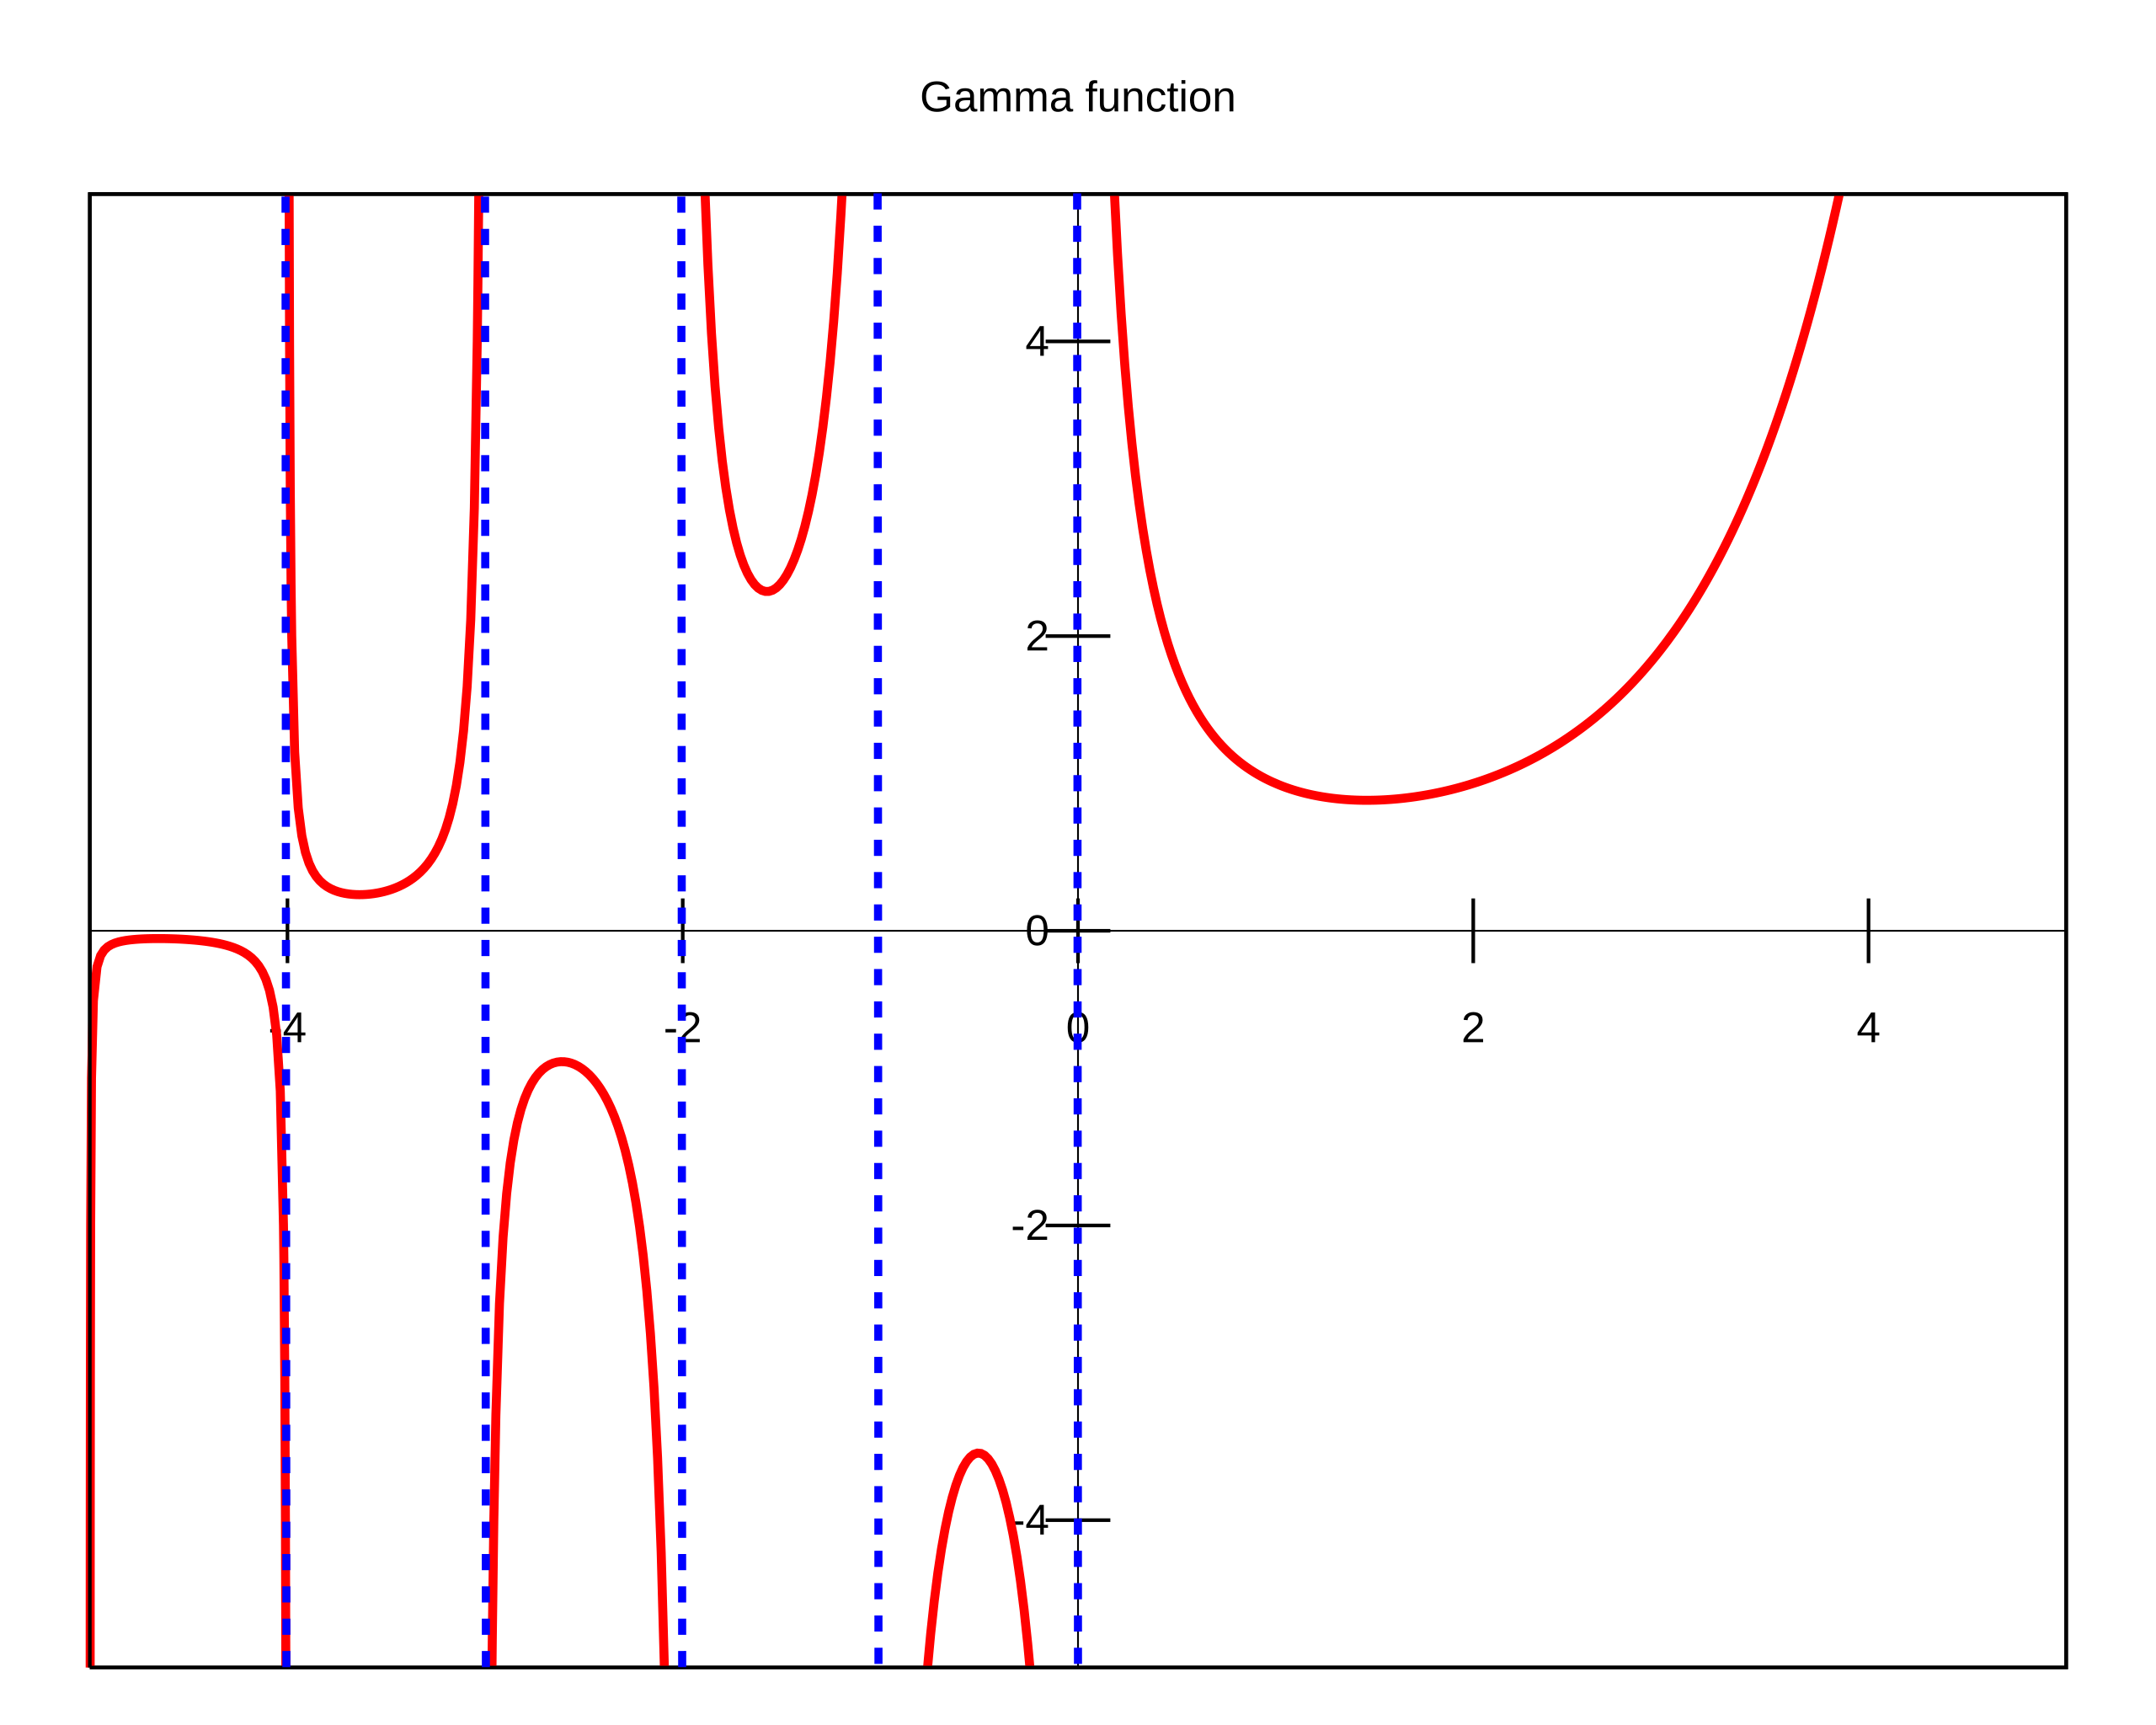
\includegraphics[width=5cm]{gamma.png}
	\begin{itemize}[label={\color{blue}$\blacktriangleright$}]
		\item The Gamma function extends factorials to real numbers
		\item Definition: $\Gamma(z) = \int_0^\infty t^{z-1}e^{-t}dt$
		\item Key property: $\Gamma(n) = (n-1)!$ for positive integers
		\item Fundamental recursive relation: $\Gamma(z+1) = z\Gamma(z)$
	\end{itemize}
\end{frame}

\begin{frame}
	\frametitle{Visualizing the Gamma Function}
	\centering
	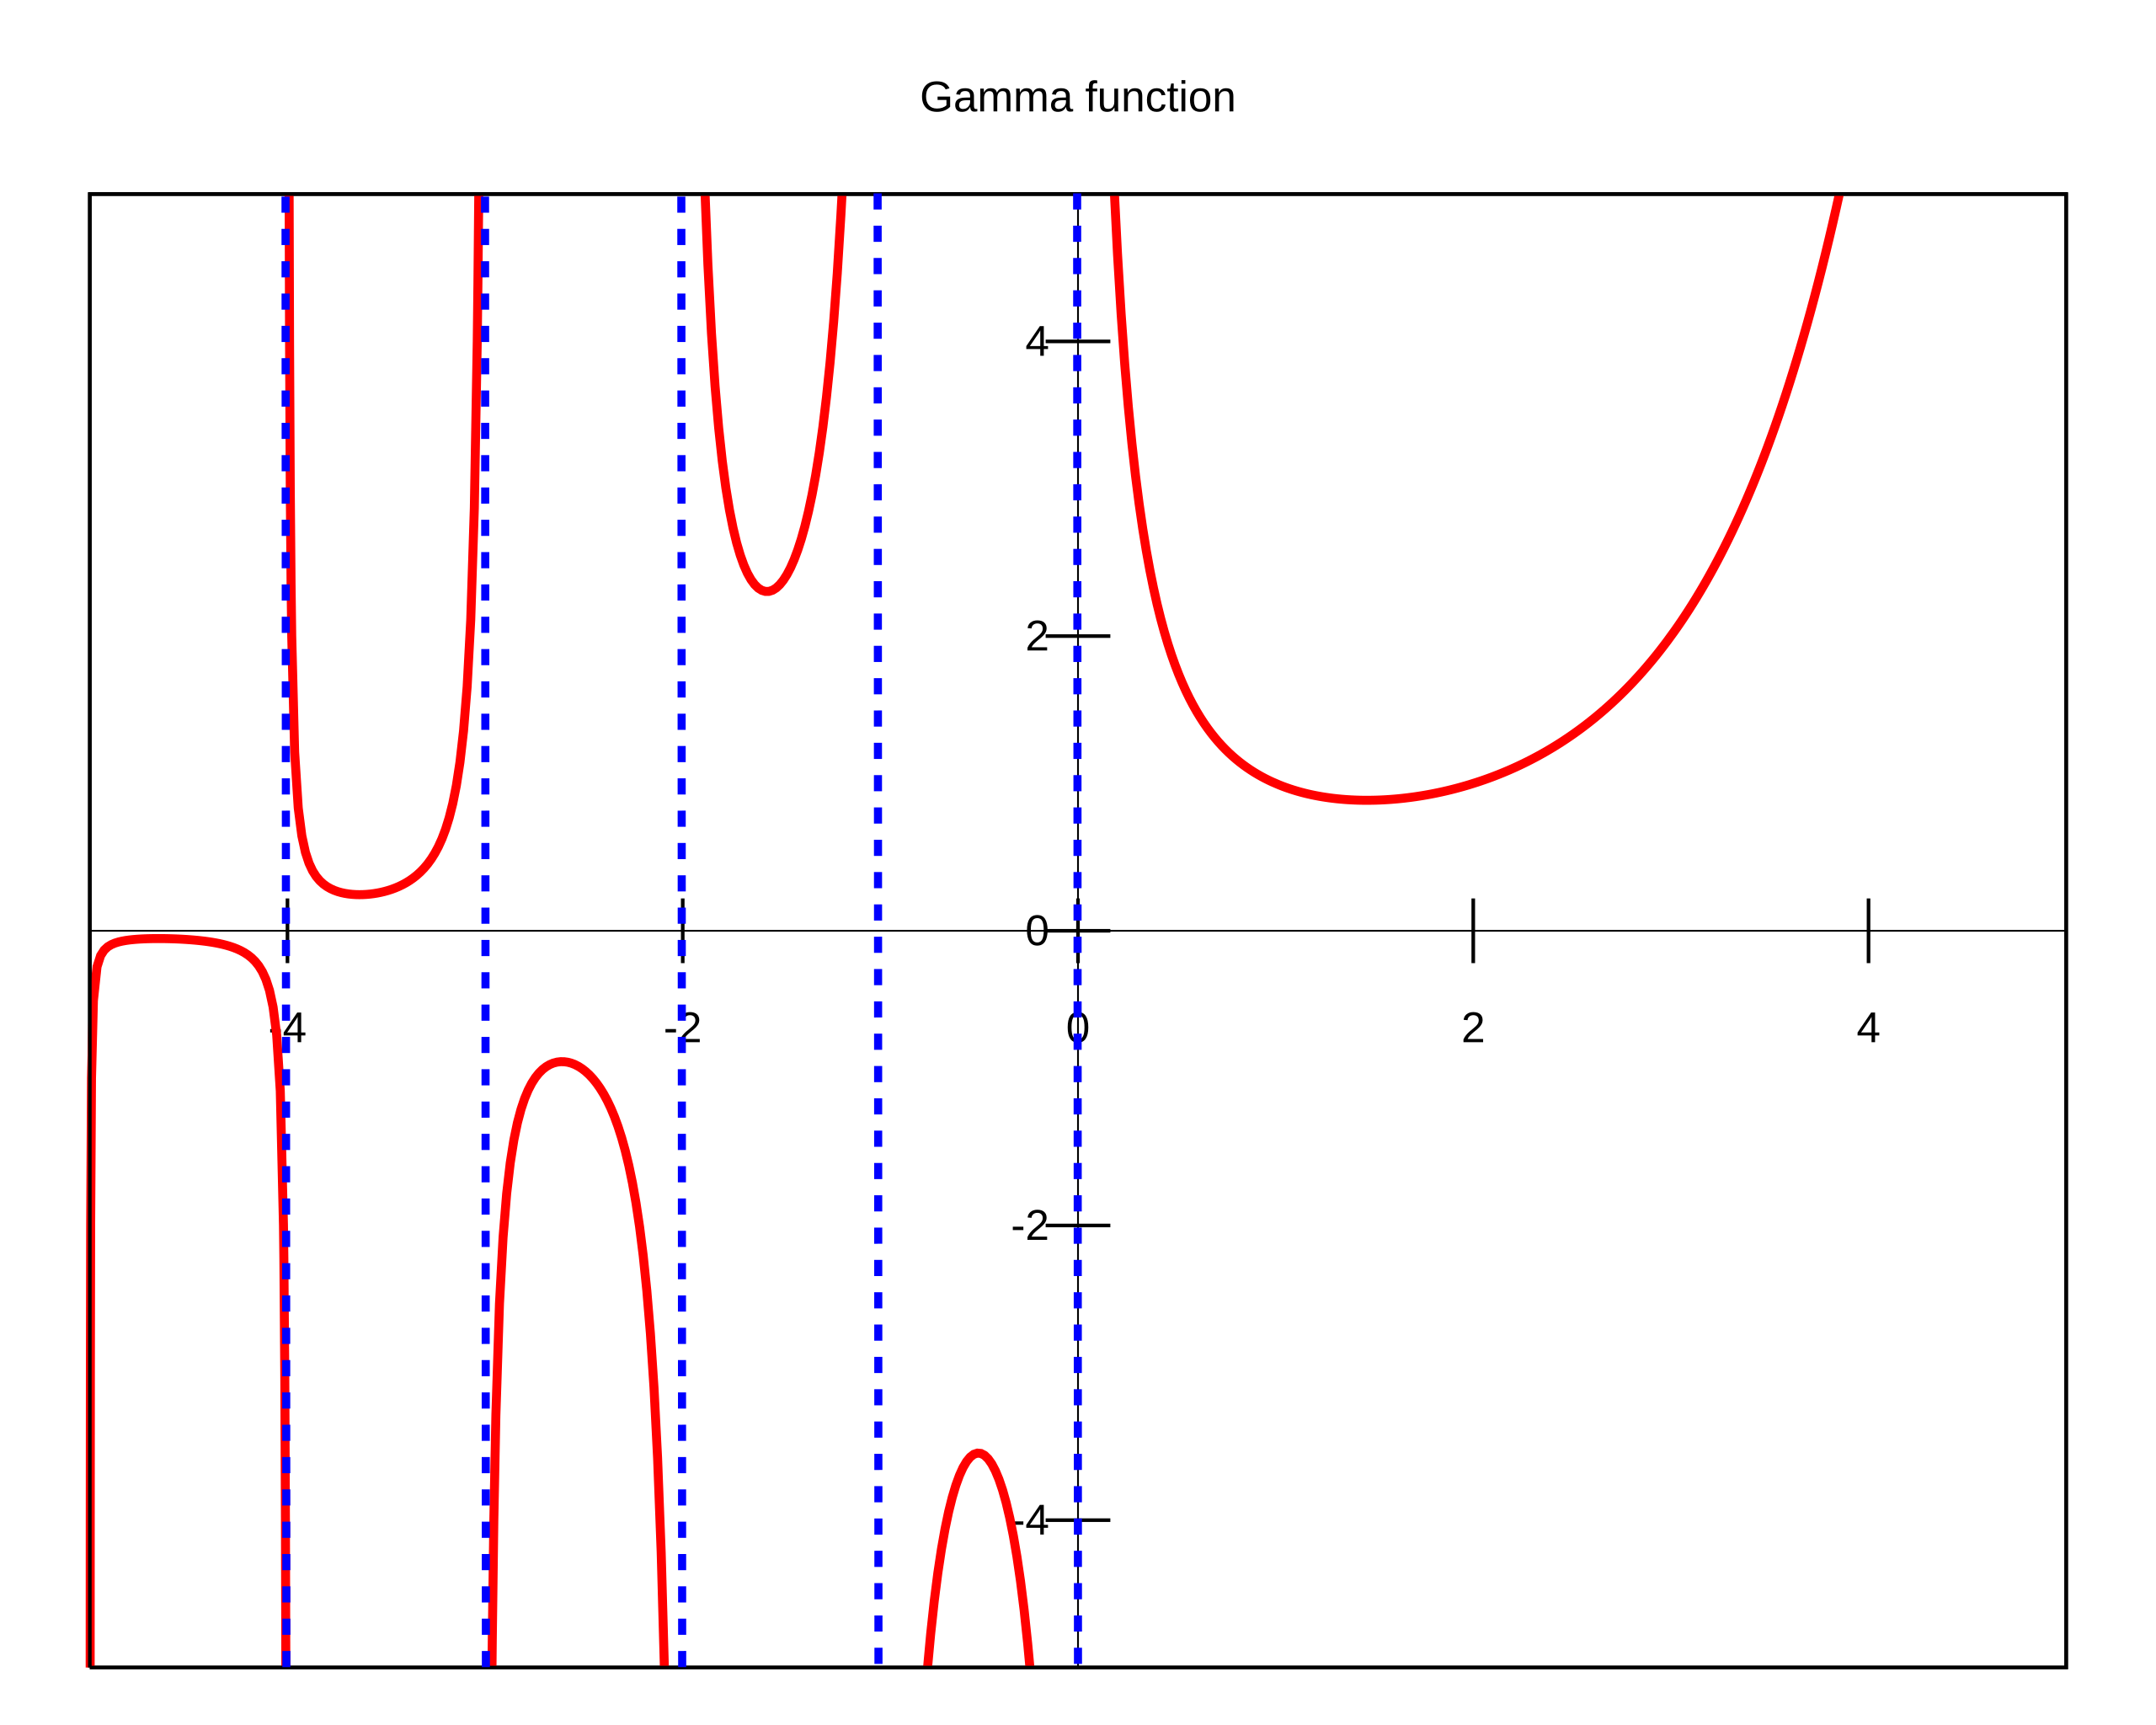
\includegraphics[width=5cm]{gamma.png}
	\begin{itemize}[label={\color{blue}$\blacktriangleright$}]
		
		\item Smooth curve through factorial points
		\item Has a minimum at $x \approx 1.46163$
		\item Poles at non-positive integers
		\item For real numbers: $\Gamma(x+1) = x\Gamma(x)$
		\item Related to many special functions in mathematics
	\end{itemize}
\end{frame}

\begin{frame}
	\frametitle{Important Properties}
	\centering
	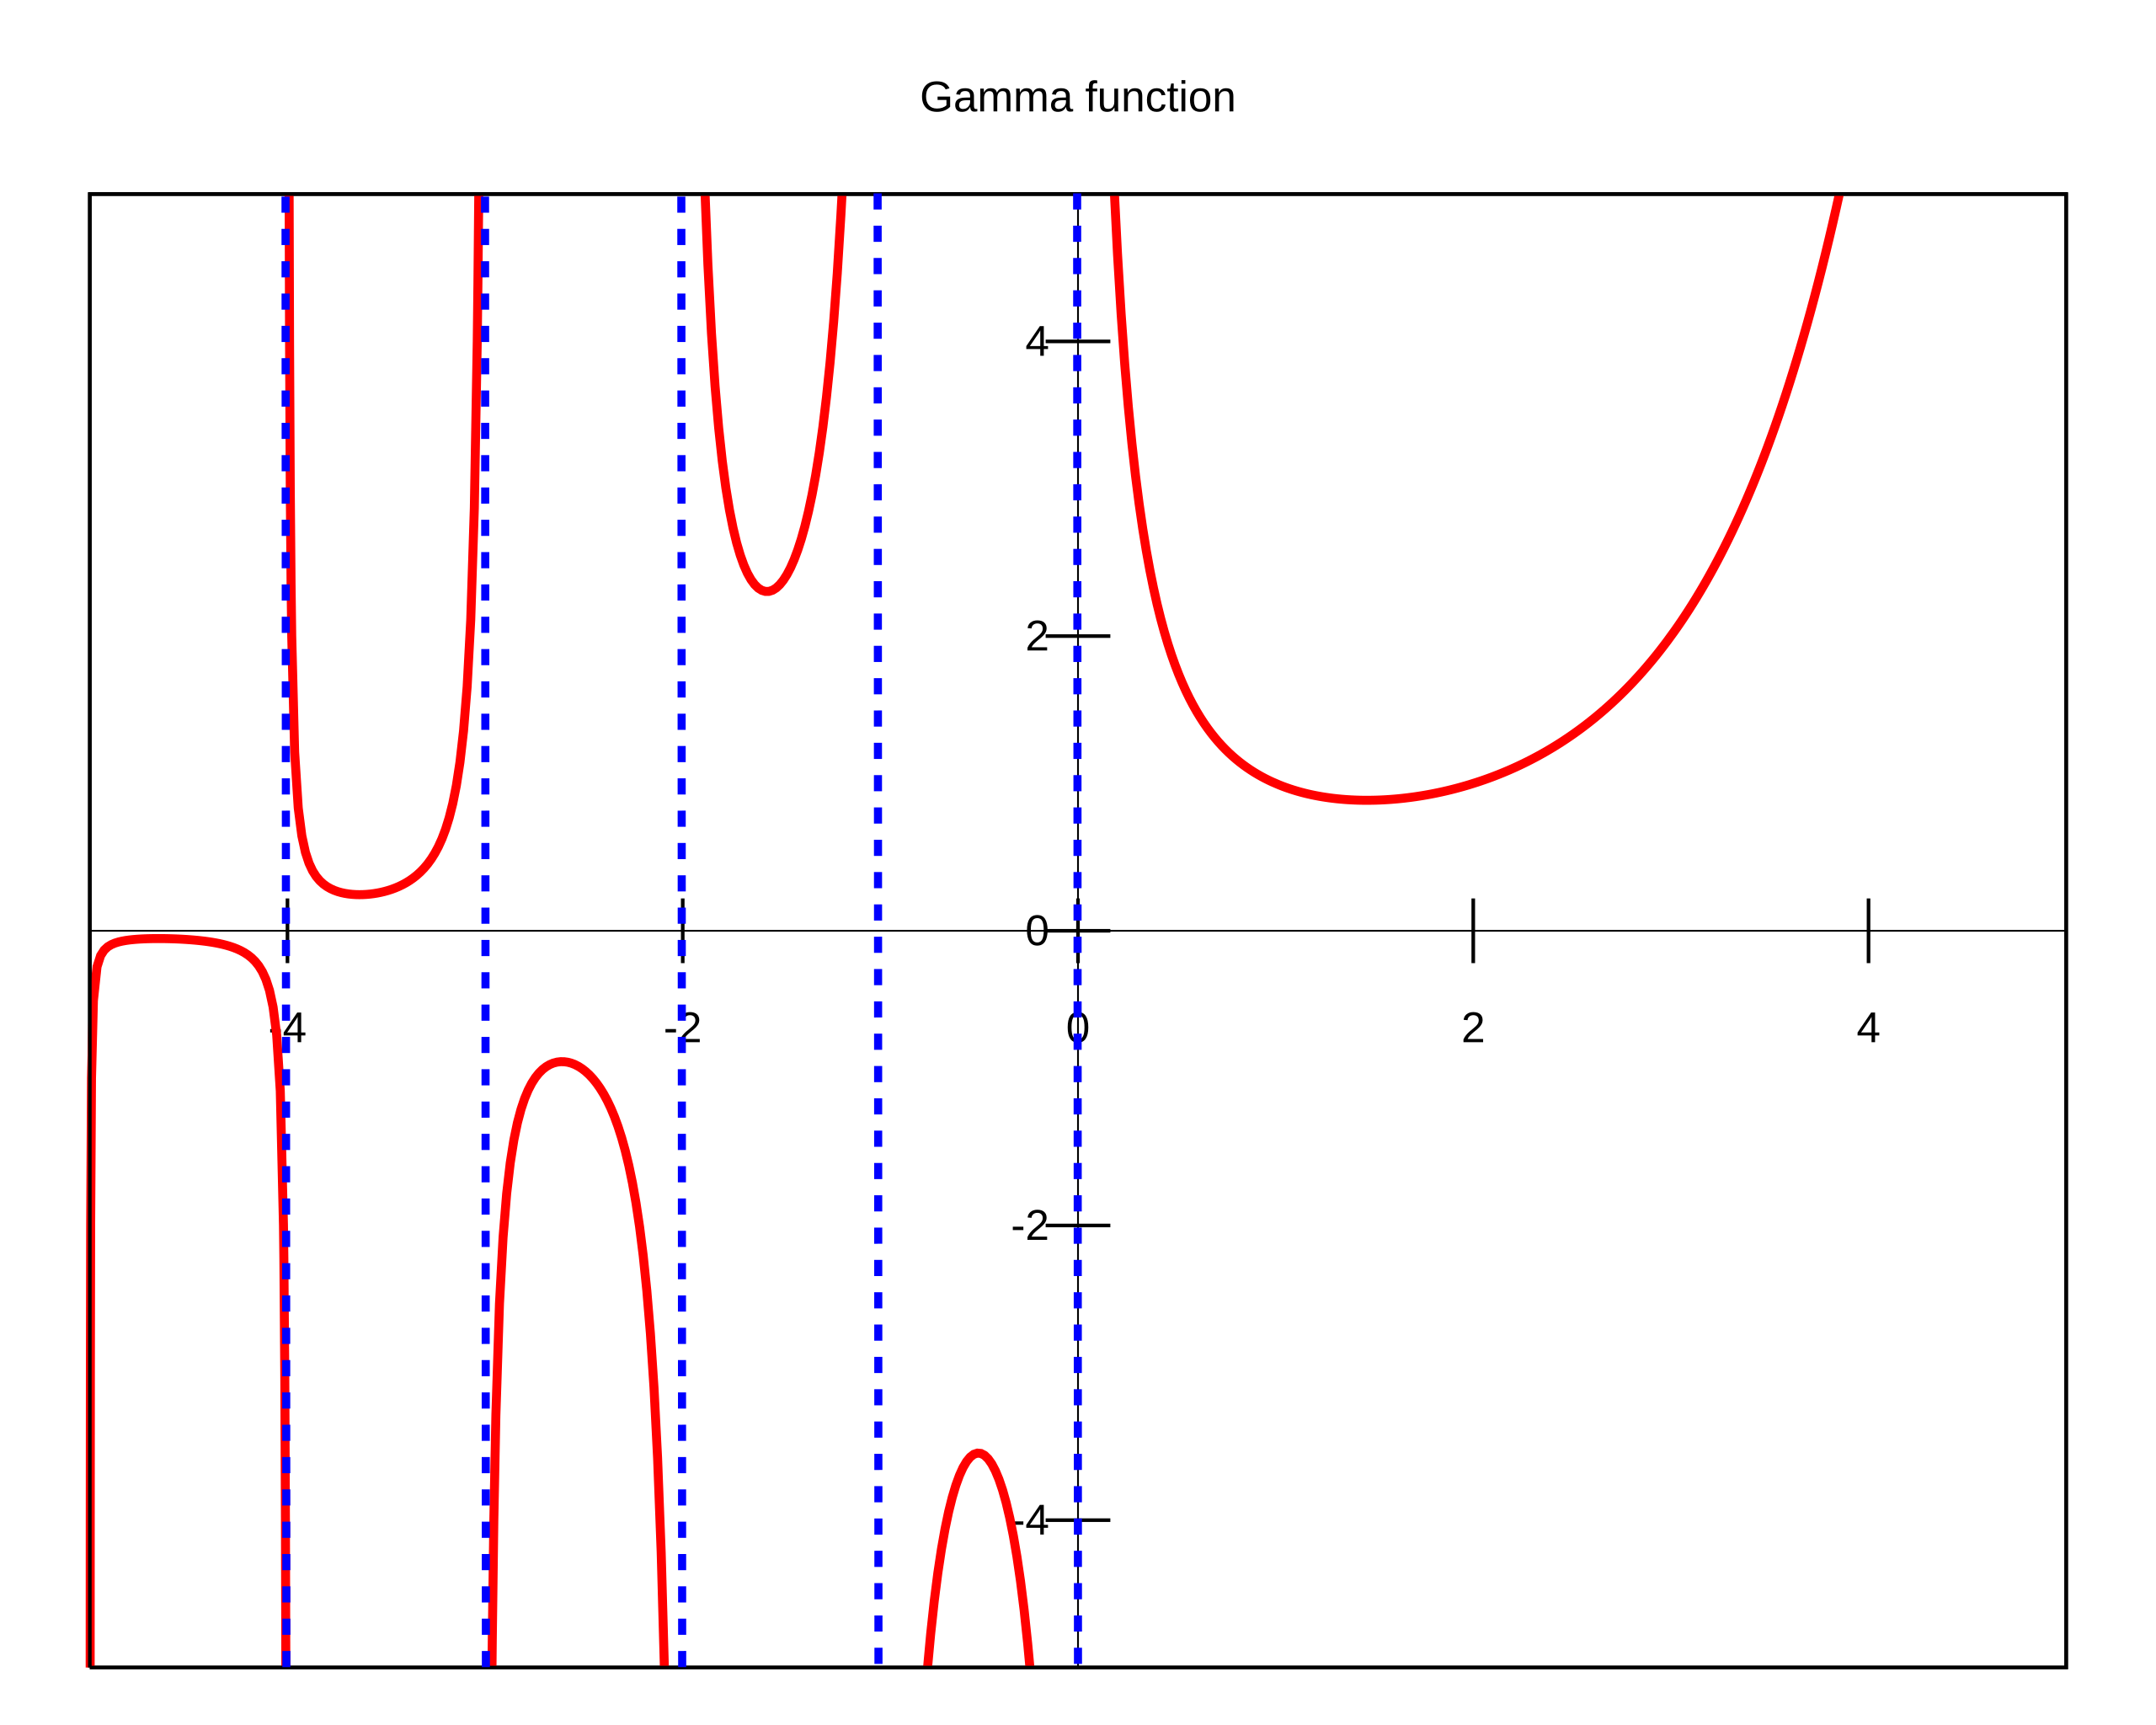
\includegraphics[width=5cm]{gamma.png}
	\begin{itemize}[label={\color{blue}$\blacktriangleright$}]
		\item Reflection formula: $\Gamma(z)\Gamma(1-z) = \frac{\pi}{\sin(\pi z)}$
		\item Special values:
		\begin{itemize}[label={\color{blue}$\blacktriangleright$}]
			\item $\Gamma(\frac{1}{2}) = \sqrt{\pi}$
			\item $\Gamma(1) = 1$
			\item $\Gamma(2) = 1$
			\item $\Gamma(n+1) = n!$ for natural numbers
		\end{itemize}
	\end{itemize}
\end{frame}

\begin{frame}
	\frametitle{Applications of the Gamma Function}
	\begin{itemize}[label={\color{blue}$\blacktriangleright$}]
		\item Statistics and Probability:
		\begin{itemize}[label={\color{blue}$\blacktriangleright$}]
			\item Gamma distribution
			\item Chi-square distribution
			\item Student's t-distribution
		\end{itemize}
		\item Physics:
		\begin{itemize}[label={\color{blue}$\blacktriangleright$}]
			\item Quantum mechanics
			\item Statistical mechanics
		\end{itemize}
	\end{itemize}
\end{frame}

\begin{frame}
	\frametitle{Application: Reliability Engineering}
	\begin{itemize}[label={\color{blue}$\blacktriangleright$}]
		\item We want to know lifetime of electronic components
		\item We can use Gamma distribution
		\begin{itemize}[label={\color{blue}$\blacktriangleright$}]
			\item Shape parameter ($k$): wear-out characteristics
			\item Scale parameter ($\theta$): time scale
			\item PDF: $f(x) = \frac{x^{k-1}e^{-x/\theta}}{\theta^k\Gamma(k)}$
			\item Helps predict failure rates and maintenance schedules
		\end{itemize}
	\end{itemize}
\end{frame}
\begin{frame}
	\frametitle{Prior: The Beta distribution}
	
	\[
	\pi(\theta) = \frac{\Gamma(\alpha + \beta)}{\Gamma(\alpha)\Gamma(\beta)}\theta^{\alpha-1}(1-\theta)^{\beta-1}
	\]
	
	
	For $0 < \theta < 1$, and zero otherwise.
	
	
	Note $\alpha > 0$ and $\beta > 0$
	
\end{frame}
\begin{frame}
	\frametitle{Beta Distribution: A Group of Shape-Shifting Distribution}
	\begin{itemize}[label={\color{blue}$\blacktriangleright$}]
		\item Beta distribution is a continuous probability distribution on interval [0,1]
		\item Two parameters: $\alpha$ (alpha) and $\beta$ (beta)
		\item Highly flexible shape: can be U-shaped, bell-shaped, or skewed
		\item Perfect for modeling probabilities and proportions
	\end{itemize}
\end{frame}

\begin{frame}
	\frametitle{Effects of Beta Parameters}
	\begin{itemize}[label={\color{blue}$\blacktriangleright$}]
		\item $\alpha = \beta = 1$: Uniform distribution
		\item $\alpha = \beta > 1$: Bell-shaped, symmetric
		\item $\alpha > \beta$: Right-skewed
		\item $\alpha < \beta$: Left-skewed
		\item Larger parameters: More concentrated distribution
		\item Mean of distribution: $\frac{\alpha}{\alpha + \beta}$
	\end{itemize}
\end{frame}

\begin{frame}
	\frametitle{Click-Through Rate Prediction for ad/email/online content}
	In Online Advertising:
	\begin{itemize}[label={\color{blue}$\blacktriangleright$}]
		\item Problem: Predicting ad click-through rates (CTR)
		\item $\alpha$ = clicks + 1
		\item $\beta$ = (views without clicks) + 1
		\item Benefits:
		\begin{itemize}[label={\color{blue}$\blacktriangleright$}]
			\item Naturally handles uncertainty
			\item Gets more accurate with more data
			\item Perfect for online learning
			\item Provides confidence intervals
		\end{itemize}
	\end{itemize}
\end{frame}

\begin{frame}
	\frametitle{Beta distribution}
	
	$Beta(\alpha,\beta)$ has density
	\[ f(\theta) = \frac{(\alpha+\beta-1)!}{(\alpha-1)!(\beta-1)!}\theta^{\alpha-1}(1-\theta)^{\beta-1} \]

	
	Observation:\\
	The coefficient is a normalizing factor, so if we have a pdf
	\[ f(\theta) = c\theta^{\alpha-1}(1-\theta)^{\beta-1} \]
	
	then
	\[ \theta \sim \text{beta}(\alpha,\beta) \]
	
	and
	\[ c = \frac{(\alpha+\beta-1)!}{(\alpha-1)!(\beta-1)!} \]
	
\end{frame}
\begin{frame}
	\frametitle{Board question preamble: beta priors}
	
	Suppose you are testing a new medical treatment with unknown probability of success $\theta$. You don't know that $\theta$, but your prior belief is that it's probably not too far from 0.5. You capture this intuition with a beta(5,5) prior on $\theta$.
	\begin{center}
		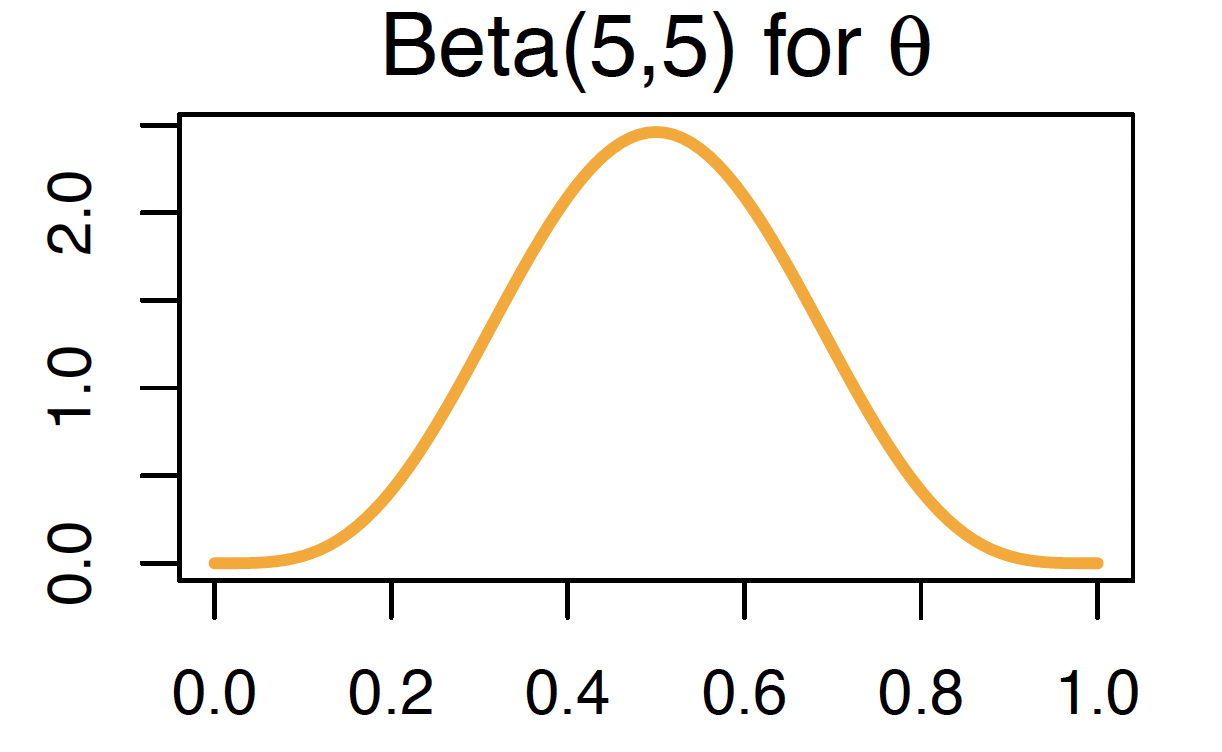
\includegraphics[width=7cm]{beta.png}
	\end{center}	

\end{frame}

\begin{frame}
	\frametitle{Board question: beta priors}
	To sharpen this distribution you take data and update the prior.
	

	\begin{itemize}[label={\color{blue}$\blacktriangleright$}]
		\item $Beta(\alpha,\beta): f(\theta) = \frac{(\alpha+\beta-1)!}{(\alpha-1)!(\beta-1)!}\theta^{\alpha-1}(1-\theta)^{\beta-1}$
		\item Treatment has prior $f(\theta) \sim \text{beta}(5,5)$
	\end{itemize}
\end{frame}
\begin{frame}
	\frametitle{Board question: beta priors}
	\begin{itemize}[label={\color{blue}$\blacktriangleright$}]
		\item Suppose you test it on 10 patients and have 6 successes. Find the posterior distribution on $\theta$. Identify the type of the posterior distribution.
		
		\item Suppose you recorded the order of the results and got SSSFFSSSSFF. Find the posterior based on this data.
		
		\item Using your answer to (2) give an integral for the posterior predictive probability of success with the next patient.
		
		\item Use what you know about pdf's to evaluate the integral without computing it directly.
	\end{itemize}
	
\end{frame}
\begin{frame}
	\frametitle{Solution}
	\begin{itemize}[label={\color{blue}$\blacktriangleright$}]
		\item 1. Prior pdf is $f(\theta) = \frac{9!}{4!4!}\theta^4(1-\theta)^4 = c_1\theta^4(1-\theta)^4$.
	\end{itemize}
	
		\begin{center}
			{\footnotesize
		\begin{tabular}{|c|c|c|c|c|}
			\hline
			hypoth. & prior & likelihood & Bayes numer. & posterior \\
			\hline
			$\theta$ & $c_1\theta^4(1-\theta)^4 d\theta$ & $\binom{10}{6}\theta^6(1-\theta)^4$ & $c_3\theta^{10}(1-\theta)^8 d\theta$ & beta(11,9) \\
			\hline
		\end{tabular}}
	\end{center}
	
	We know the normalized posterior is a beta distribution because it has the form of a beta distribution ($c\theta^{a-1}(1-\theta)^{b-1}$ on [0,1]) so by our earlier observation it must be a beta distribution.
	\begin{itemize}[label={\color{blue}$\blacktriangleright$}]
	\item 2. The answer is the same. The only change is that the likelihood has a coefficient of 1 instead of a binomial coefficient.
	
	\item 3. The posterior on $\theta$ is beta(11,9) which has density
	\[ f(\theta|\text{data}) = \frac{19!}{10!8!}\theta^{10}(1-\theta)^8. \]
\end{itemize}
\end{frame}
\begin{frame}
	\frametitle{Solution continued}
	
	The law of total probability says that the posterior predictive probability of success is
	
	\[ P(\text{success}|\text{data}) = \int_0^1 f(\text{success}|\theta) \cdot f(\theta|\text{data}) d\theta \]
	\[ = \int_0^1 \theta \cdot \frac{19!}{10!8!}\theta^{10}(1-\theta)^8 d\theta = \int_0^1 \frac{19!}{10!8!}\theta^{11}(1-\theta)^8 d\theta \]
\end{frame}
\begin{frame}
	\frametitle{Solution continued}
	4. We compute the integral in (3) by relating it to the pdf of beta(12,9): $\frac{20!}{11!8!}\theta^{11}(1-\theta)^7$. Since the pdf of beta(12,9) integrates to 1 we have
	
	\[ \int_0^1 \frac{20!}{11!8!}\theta^{11}(1-\theta)^7 = 1 \quad \Rightarrow \quad \int_0^1 \theta^{11}(1-\theta)^7 = \frac{11!8!}{20!}. \]
	
	Thus
	\[ \int_0^1 \frac{19!}{10!8!}\theta^{11}(1-\theta)^8 d\theta = \frac{19!}{10!8!} \cdot \frac{11!8!}{20!} = \boxed{\frac{11}{20}}. \]
	
\end{frame}
\begin{frame}
	\frametitle{Conjugate priors}
	
	We had
	\begin{itemize}[label={\color{blue}$\blacktriangleright$}]
		\item Prior $f(\theta) d\theta$: \textcolor{blue}{beta distribution}
		\item Likelihood $p(x|\theta)$: binomial distribution
		\item Posterior $f(\theta|x) d\theta$: \textcolor{blue}{beta distribution}
	\end{itemize}
	
	The beta distribution is called a \textcolor{blue}{conjugate prior} for the binomial likelihood.
	
	That is, the beta prior becomes a beta posterior and repeated updating is easy!
	
\end{frame}

\begin{frame}
	\frametitle{Beta prior: $\pi(\theta) = \frac{\Gamma(\alpha+\beta)}{\Gamma(\alpha)\Gamma(\beta)}\theta^{\alpha-1}(1-\theta)^{\beta-1}$}
	
	\begin{itemize}[label={\color{blue}$\blacktriangleright$}]
		\item Supported on $[0,1]$.
		
		\item $E(\theta) = \frac{\alpha}{\alpha+\beta}$
		
		\item $Var(\theta) = \frac{\alpha\beta}{(\alpha+\beta)^2(\alpha+\beta+1)}$.
		
		\item Can assume a variety of shapes depending on $\alpha$ and $\beta$.
		
		\item When $\alpha = \beta = 1$, it's uniform.
		
		\item Bayes used a Bernoulli model and a uniform prior in his posthumous paper.
	\end{itemize}
	
\end{frame}
\begin{frame}
	\frametitle{Posterior Distribution}
	
	\begin{align*}
		\pi(\theta|x) &\propto p(x|\theta)\,\pi(\theta) \\[1em]
		&= \theta^{\sum_{i=1}^n x_i}(1-\theta)^{n-\sum_{i=1}^n x_i}\frac{\Gamma(\alpha+\beta)}{\Gamma(\alpha)\Gamma(\beta)}\theta^{\alpha-1}(1-\theta)^{\beta-1} \\[1em]
		&\propto \theta^{(\alpha+\sum_{i=1}^n x_i)-1}(1-\theta)^{(\beta+n-\sum_{i=1}^n x_i)-1}
	\end{align*}
	
	Proportional to the density of a Beta($\alpha'$, $\beta'$), with
	\[
	\begin{aligned}
		\alpha' &= \alpha + \sum_{i=1}^n x_i \\
		\beta' &= \beta + n - \sum_{i=1}^n x_i
	\end{aligned}
	\]
	
\end{frame}
\begin{frame}
	\frametitle{Conjugate Priors}
	
	\begin{itemize}[label={\color{blue}$\blacktriangleright$}]
		\item Prior was Beta($\alpha$, $\beta$).
		\item Posterior is Beta($\alpha'$, $\beta'$).
		\item Prior and posterior are in the same family of distributions.
		\item The Beta is a \textit{conjugate prior} for the Bernoulli model.
		\item Posterior was obtained by inspection.
		\item Conjugate priors are very convenient.
		\item There are conjugate priors for many models.
		\item There are also important models for which conjugate priors do not exist.
	\end{itemize}
	
\end{frame}
\begin{frame}
	\frametitle{Concept Question}
	
	Suppose your prior $f(\theta)$ in the bent coin example is Beta(6,8). You flip the coin 7 times, getting 2 heads and 5 tails. What is the posterior pdf $f(\theta|x)$?
	
	\begin{itemize}[label={\color{blue}$\blacktriangleright$}]
		\item Beta(2,5)
		\item Beta(3,6)
		\item Beta(6,8)
		\item Beta(8,13)
	\end{itemize}
	
	We saw in the previous board question that 2 heads and 5 tails will update a beta$(\alpha,\beta)$ prior to a beta$(\alpha+2,\beta+5)$ posterior.
	
	\medskip
	\textbf{answer:} (4) beta(8,13).
	
\end{frame}
\begin{frame}
	\frametitle{Continuous priors, continuous data}
	
	Bayesian update tables:
	\begin{center}
		\begin{tabular}{ccccc}
			\toprule
			& & & Bayes & posterior \\
			hypoth. & prior & likelihood & numerator & $f(\theta|x) d\theta$ \\
			\midrule
			$\theta$ & $f(\theta) d\theta$ & $f(x|\theta)$ & $f(x|\theta)f(\theta) d\theta$ & $\frac{f(x|\theta)f(\theta) d\theta}{f(x)}$ \\
			\midrule
			total & 1 & & $f(x)$ & 1 \\
			\bottomrule
		\end{tabular}
	\end{center}
	
	\[ f(x) = \int f(x|\theta)f(\theta) d\theta \]
	
\end{frame}
\begin{frame}
	\frametitle{Picture of the posterior}
	
	Suppose 60 out of 100 consumers picked the new blend of coffee beans.
	
	Posterior is Beta, with $\alpha' = \alpha + \sum_{i=1}^n x_i = 61$ and 
	$\beta' = \beta + n - \sum_{i=1}^n x_i = 41$.
	
	\begin{center}
	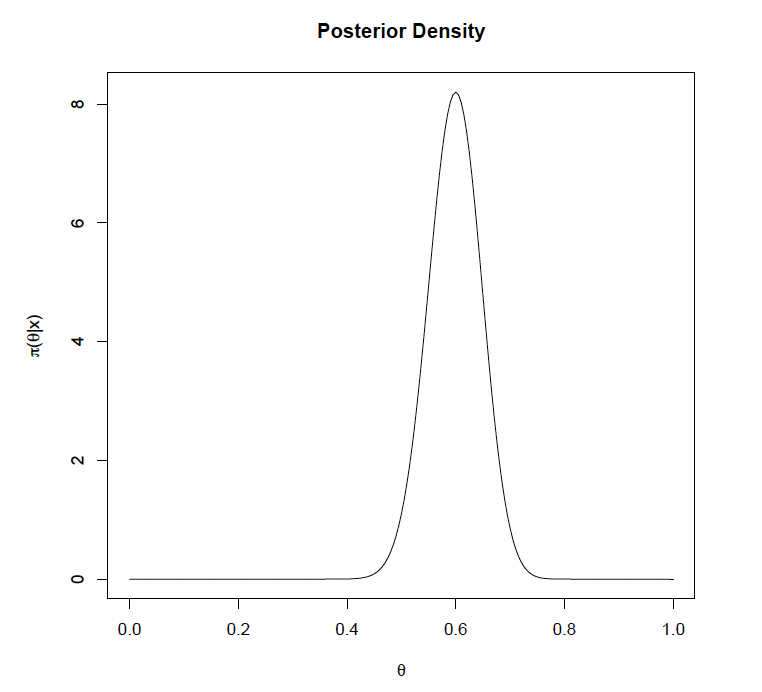
\includegraphics[width=6cm]{post.png}
	\end{center}
	
\end{frame}

\end{document}